\documentclass{beamer}
\usepackage[utf8]{inputenc}
\usepackage[T1]{fontenc}
\usepackage[polish]{babel}
\usepackage{amsmath}
\usepackage{ulem}

\renewcommand<>{\sout}[1]{
    \alt#2{\beameroriginal{\sout}{#1}}{#1}
}

% \includeonlyframes{current}


\newcommand{\n}{\,\\}

\usetheme{Boadilla}

\title{Początki Lispu}
\subtitle{(((Archeologia Cyfrowa)))}
\author{Jakub Grobelny}
\date{19.11.2019}

\begin{document}

%==============================================================================%

\begin{frame}
\titlepage
\end{frame}

\begin{frame}
\frametitle{O czym będzie?}
\tableofcontents
\end{frame}

%==============================================================================%

\section{Do czego był potrzebny taki język?}
\begin{frame}
\frametitle{Narodziny sztucznej inteligencji}
\pause
Lata 50. XX wieku były czasem, gdy sztuczna inteligencja pojawiła się jako 
dziedzina wiedzy.
\pause
\begin{description}
    \item[1950] Alan Turing publikuje ,,\textit{Computing Machinery 
                and Intelligence}''
        \begin{itemize}
            \item \pause 
                \only<-5>{,,\textit{Czy maszyny myślą?}''}
                \only<6-8>{\sout{,,\textit{Czy maszyny myślą?}''}}
            \item \pause 
                \only<-5>{,,\textit{Czy maszyny mogą myśleć?}''}
                \only<6-8>{\sout{,,\textit{Czy maszyny mogą myśleć?}''}}
            \item \pause,,\textit{Czy maszyny mogą działać nieodróżnialnie od ludzi?}''
        \end{itemize} \pause
    \item[1951] Marvin Lee Minsky buduje sieć neuronową 
                SNARC\footnotemark\pause
    \item[1951] Pierwsze programy grające w warcaby (Christopher 
                Strachey) i szachy (Dietrich Prinz)
\end{description}
\only<7-8>{\footnotetext[1]{Stochastic neural analog reinforcement calculator}}
\end{frame}

\begin{frame}
\frametitle{Narodziny sztucznej inteligencji}
\begin{description}
    \item[1955] Allen Newell, Herbert A. Simon i Cliff Shaw
                tworzą program ,,\textit{Logic Theorist}'' \pause
        \begin{itemize}
            \item Program naśladujący ludzkie techniki rozwiązywania 
                  problemów \pause
            \item Program manipulujący \textbf{symbolami} \pause
            \item Udowodnił 38 z pierwszych 52 twierdzeń z ,,\textit{Principia 
                  Mathematica}''\footnotemark \pause \,(niektóre z dowodów były 
                  bardziej eleganckie niż wcześniej istniejące)... \pause
            \item ...i to wszystko zanim określenie ,,sztuczna inteligencja'' w 
            ogóle zostało stworzone.
        \end{itemize}
\end{description}

\only<4-6>{\footnotetext[2]{Autorstwa Alfreda Northa Whiteheada i Bertranda 
                            Russella}}
\end{frame}


\begin{frame}
\frametitle{Narodziny sztucznej inteligencji}

\begin{columns}
\column{0.5\textwidth}

\begin{description}
    \item[1956] Konferencja w Dartmouth. \pause
                \textbf{John McCarthy} przekonuje zebranych do
                używania terminu ,,\textit{sztuczna inteligencja}''.
\end{description}

\column{0.5\textwidth}
\begin{figure}
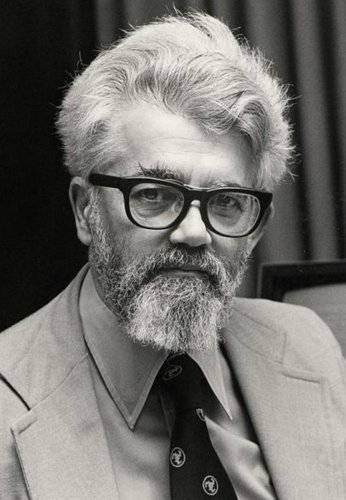
\includegraphics[scale=1.2]{images/mccarthy.jpg}
\caption{John McCarthy}
\end{figure}
\end{columns}
\end{frame}


\begin{frame}
\frametitle{Symbole}
\pause
Okazuje się, że operowanie na \textbf{symbolach} jest istotne przy 
tworzeniu sztucznej inteligencji. \pause

\n Ludzkie rozumowanie opiera się na manipulacji symbolami (\textit{physical symbol system hypothesis} -- Allan Newell i Herbert A. Simon)\pause

\n System symboli składa się z symboli, składania ich w struktury (wyrażenia) i manipulowania nimi (przetwarzania) w celu tworzenia nowych wyrażeń.

\end{frame}


\begin{frame}
\frametitle{Symbole}

W 1959 roku John McCarthy pisze pracę ,,\textit{Programs with common sense}''.
\pause

\n Proponuje w niej stworzenie programu ,,\textit{Advice Taker}'', który rozwiązywałby problemy poprzez manipulację zdaniami (\textbf{symbole!}).
\pause

\n ,,\textit{Our ultimate objective is to make programs that 
              learn from their experience as effectively
              as humans do.}''
\end{frame}



\begin{frame}
\frametitle{,,\textit{Programs with common sense}''}
\pause
,,\textit{A class of entities called terms
is defined and a term is an expression. A sequence of expressions is an 
expression. These expressions are represented in the machine by list 
structures}'' -- reprezentacja przesłanek/faktów w postaci \textbf{list symboli}
\end{frame}

\begin{frame}
Przykłady:
\pause
    $$at(I, desk)$$
    $$at(desk, home)$$
    $$at(car, home)$$
    $$at(home, county)$$
    $$at(airport, county)$$
\pause
    $$at(x, y), at(y,z) \rightarrow at(x,z)$$
\pause
    $$transitive(at)$$
    $$transitive(u) \rightarrow (u(x,y), u(y,z) \rightarrow u(x,z))$$
\pause
Prawie jak Prolog?
\end{frame}
    


\begin{frame}[fragile]
\frametitle{Zapotrzebowanie na nowe języki}

\begin{columns}
\column{0.6\textwidth}
\textbf{Information Processing Language} \normalsize -- niskopozimowy język 
programowania do manipulowania listami stworzony przez Newella, Shawa i Simona, 
który posłużył do napisania programu. ,,\textit{Logic Theorist}''.
\pause
\n \n Dwa rodzaje wyrażeń:
\begin{itemize}
    \item dane reprezentowane jako listy
    \item procedury operujące na danych
\end{itemize}

\column{0.4\textwidth}
\begin{figure}
\begin{verbatim}
     IPL-V  List 
      Structure 
       Example
    Name SYMB LINK
    L1   9-1  100
    100  S4   101
    101  S5   0
    9-1  0    200
    200  A1   201
    201  V1   202
    202  A2   203
    203  V2   0

\end{verbatim}
\caption{Lista zapisana w IPL-V}
\end{figure}
\end{columns}
\end{frame}


\begin{frame}
\frametitle{Information Processing Language}
Nowe feature'y:\pause

\begin{itemize}
    \item Manipulacja listami (tylko listy atomów)\pause
    \item Funkcje wyższego rzędu\pause
    \item Obliczenia na symbolach (tylko litera+liczba)\pause
\end{itemize}

\n Alternatywy?\pause\, Brak.

\end{frame}


%==============================================================================%

\section{,,\textit{Recursive Functions of Symbolic Expressions...}''}

\begin{frame}
\frametitle{Wymyślenie Lispu}
\pause
W 1960 ukazuje się praca Johna McCarthy'ego pt.,,\textit{Recursive Functions of Symbolic Expressions
Their Computation by Machine, Part I}''. \pause
\begin{figure}
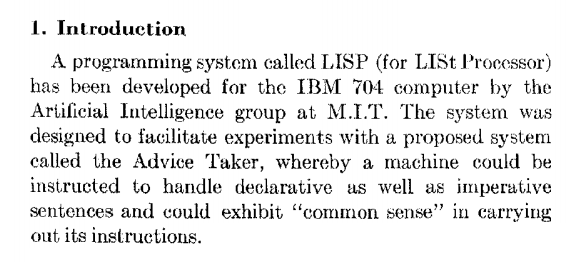
\includegraphics[scale=2.3]{images/recursive-functions-1.png}
\end{figure}
\end{frame}


\begin{frame}
\frametitle{Cele}
\pause
\begin{itemize}
    \item Lisp został wymyślony ze względu na ,,\textit{Advice Taker'a}''.\pause
    \item Języka programowania do manipulacji wyrażeniami reprezentującymi 
    zdania, przy użyciu których ,,\textit{Advice Taker}'' mógłby 
    przeprowadzać wnioskowania.
\end{itemize}
\end{frame}


\begin{frame}
\frametitle{Wyrażenia warunkowe}
\pause
Po raz pierwszy pojawiła się idea \textit{wyrażeń warunkowych}.
\pause

\begin{figure}
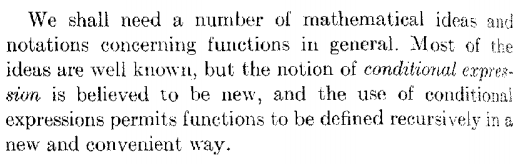
\includegraphics[scale=0.6]{images/conditional.png}
\end{figure}
\pause

Wyrażenia warunkowe są następującej postaci:
$$(p_1 \rightarrow e_1,\,...\, p_n \rightarrow e_n)$$
\end{frame}


\begin{frame}
\frametitle{Wyrażenia warunkowe}

Wyrażenia warunkowe są następującej postaci:
$$(p_1 \rightarrow e_1,\,...\, p_n \rightarrow e_n)$$

Interpretacja:
\pause
\n ,,Jeżeli $p_1$ to $e_1$, w przeciwnym razie jeżeli $p_2$ to $e_2$, \,...\,, w przciwnym razie jeżeli $p_n$ to $e_n$''
\pause
\n \n lub
\pause
\n 
,,$p_1$ daje $e_1$, \,...\,, $p_n$ daje $e_n$''

\end{frame}


\begin{frame}
\frametitle{Wyrażenia warunkowe}
Zasady obliczania wartości wyrażeń warunkowych:
\begin{itemize}
    \item \pause Rozpatruj $p$ od lewej do prawej.
    \item \pause Jeżeli $p$, którego wartość to $T$, występuje przed 
                 jakimkolwiek innym $p$, którego wartość jest niezdefiniowana, 
                 to wartością wyrażenia warunkowego jest wartość 
                 odpowiadającego $e$ (jeżeli jest zdefiniowane).
    \item \pause Jeżeli jakiekolwiek niezdefiniowane $p$ jest napotkane przed 
                 prawdziwym $p$, lub gdy wszystkie $p$ są fałszywe, bądź gdy 
                 $e$ odpowiadającego pierwszemu prawdziwemu $p$ jest 
                 niezdefiniowane, to wartość wyrażenia jest niezdefiniowana.
\end{itemize}
\end{frame}

\begin{frame}
\frametitle{Wyrażenia warunkowe}
Przykłady:\pause

$$(2 < 1 \rightarrow 4, T \rightarrow 3) = \pause 3$$\pause
$$(2 < 1 \rightarrow \frac{0}{0}, T \rightarrow 3) = \pause 3$$\pause
$$(2 < 1 \rightarrow 3, T \rightarrow \frac{0}{0}) = \pause undefined$$\pause
$$(2 < 1 \rightarrow 3, 4 < 1 \rightarrow 1) = \pause undefined$$
\end{frame}


\begin{frame}
\frametitle{Wyrażenia warunkowe}

Wyrażenia warunkowe pozwalają na eleganckie zapisywanie funkcji:
\pause
$$|x| = (x < 0 \rightarrow -x, T \rightarrow x)$$
\pause
$$sgn(x) = (x < 0 \rightarrow -1, x = 0 \rightarrow 0, T \rightarrow 1)$$
\end{frame}


\begin{frame}
\frametitle{Funkcje rekurencyjne}

Bardzo zwięzły staje się też zapis funkcji rekurencyjnych:
\pause
$$n! = (n = 0 \rightarrow 1, T \rightarrow n \cdot (n - 1)!)$$
\pause
\begin{equation*}
\begin{gathered}
    gcd(m ,n) = (m > n \rightarrow gcd(n,m), \\
                rem(n,m) = 0\rightarrow m, \\
                T \rightarrow gcd(rem(n,m), m))
\end{gathered}
\end{equation*}
\end{frame}


\begin{frame}
\frametitle{Funkcje rekurencyjne}
\begin{figure}
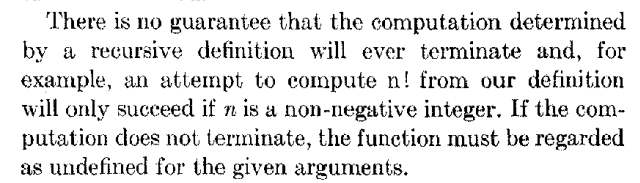
\includegraphics[scale=2.20]{images/infinite-recursion.png}
\end{figure}
\end{frame}


\begin{frame}
\frametitle{Spójniki logiczne}
\pause
$$p \wedge q = (p \rightarrow q, T \rightarrow F)$$
$$p \vee q = (p \rightarrow T, T \rightarrow q)$$
$$ \sim{p} = (p \rightarrow F, T \rightarrow T)$$
$$p \Rightarrow q = (p \rightarrow q, T \rightarrow T)$$
\end{frame}


\begin{frame}
\frametitle{Spójniki logiczne}
\begin{figure}
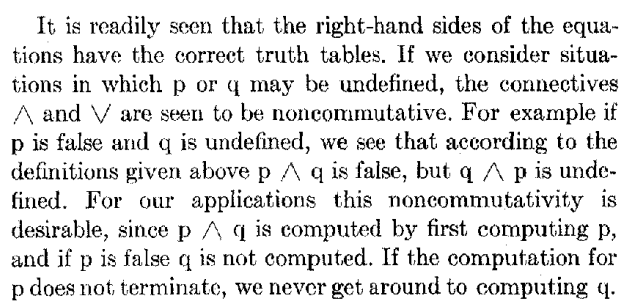
\includegraphics[scale=2.1]{images/lazy.png}
\caption{Ewaluacja leniwa?}
\end{figure}
\end{frame}


\begin{frame}
\frametitle{Spójniki logiczne}
$$ p \wedge q = (p \rightarrow q, T \rightarrow F)$$
Argumenty funkcji ,,$\wedge$'' nie są poddawane ewaluacji przed jej aplikacją.
\end{frame}


\begin{frame}
\frametitle{Formy a funkcje}
\pause
Pojęcie formy zostało zapożyczone z rachunku lambda Churcha.

\pause
\n $y^2 + x$ -- forma


\pause
$(y^2 + x)(3,4)$ -- źle. Nie wiadomo czy wartością powinno być 13 czy 19.

\pause
\n Formę $\mathcal{E}$ możemy skonwertować na funkcję jeżeli ustalimy powiązanie między zmiennymi w formie a uporządkowaną listą argumentów funkcji:

\pause
\n $\lambda((x_1,\,...\,,x_n), \mathcal{E}))$ -- funkcja


\pause
$\lambda((x, y), y^2 + x)$ -- też funkcja
\end{frame}


\begin{frame}
\frametitle{Rekurencyjne $\lambda$-wyrażenia}
\pause

\begin{equation*}
    \begin{gathered}
    sqrt = \lambda((a,x,\epsilon),\\
        (|x^2 - a| < \epsilon \rightarrow x, 
        T \rightarrow sqrt(a, \frac{1}{2}(x + \frac{a}{x}), \epsilon)))
    \end{gathered}
\end{equation*}

\pause
Prawa strona wyrażenia nie może być wyrażeniem dla tej funkcji, bo nic nie wskazuje na to, że $sqrt$ do odnosi się do całego wyrażenia ($sqrt$ nie jest związane).


\pause
\n Operator punktu stałego? \pause-- zbyt długie i nieczytelne wyrażenia.

\end{frame}


\begin{frame}
\frametitle{Rekurencyjne $\lambda$-wyrażenia}

Nowa notacja:
\pause

$$label(a, \mathcal{E})$$
\pause

Wyrażenie $\mathcal{E}$, w którym wszystkie wystąpienia $a$ interpretowane są jako odniesienia do całego wyrażenia $\mathcal{E}$.
\pause
\end{frame}


\begin{frame}
\frametitle{S-wyrażenia}
\pause

,,\textit{A Class of Symbolic Expressions}''.
\pause

\n Dopuszczalne znaki:
\begin{itemize}
    \item $.$ \pause
    \item $)$ \pause
    \item $($ \pause
    \item Nieskończony zbiór rozróżnialnych symboli atomowych -- napisów złożonych z wielkich liter alfabetu łacińskiego, cyfr i pojedynczych spacji.
    \pause\n Na przykład:
        \begin{itemize}
            \item A
            \item ABA
            \item APPLE PIE NUMBER 3
        \end{itemize}
\end{itemize}
\end{frame}



\begin{frame}
\frametitle{S-wyrażenia}
Czemu symbole składające się z wielu znaków?\pause

\n Odpowiedź:
\begin{itemize}
    \item IBM 704 miał tylko 47 drukowalnych znaków \pause
    \item Nazywanie atomowych bytów angielskimi słowami i zdaniami jest wygodne

\end{itemize}
\end{frame}


\begin{frame}
\frametitle{S-wyrażenia}

Definicja indukcyjna S-wyrażeń:

\begin{enumerate}
    \item\pause Symbole atomowe są S-wyrażeniami
    \item\pause Jeżeli $e_1$ i $e_2$ są S-wyrażeniami, to $(e_1 \cdot e_2)$ 
                również jest S-wyrażeniem.
\end{enumerate}

\pause \n Przykładowe S-wyrażenia:
$$AB$$
$$(A \cdot B)$$
$$((AB \cdot C) \cdot D)$$
\end{frame}


\begin{frame}
\frametitle{Listy (S-wyrażenia)}

Możemy reprezentować listy dowolnej długości przy użyciu S-wyrażeń w następujący sposób:

\pause \n
$(m_1, m_2, \,...\, m_n) = (m_1 \cdot (m_2 \cdot (...(m_n \cdot NIL)...)))$
\pause

Gdzie NIL jest specjalnym symbolem kończącym listy.

\pause \n
Wprowadzamy zatem specjalną notację dla list:\pause
\begin{enumerate}
    \item $(m) = (m \cdot NIL)$
    \item $(m_1, m_2, \,...\, m_n) = 
           (m_1 \cdot (...(m_n \cdot NIL)...))$
    \item $(m_1, \,...\, ,m_n \cdot x) = (m_1 \cdot (...(m_n \cdot x)...))$
\end{enumerate}
\end{frame}


\begin{frame}
\frametitle{M-wyrażenia}
\pause
Aby odróżnić wyrażenia reprezentujące aplikację funkcji od S-wyrażeń, będziemy małych liter do nazywania funkcji i zmiennych.


\pause \n
Będziemy również używać nawiasów kwadratowych i średników zamiast nawiasów i przecinków.

\pause
Na przykład:
$$car[x]$$
$$car[cons[(A \cdot B); x]]$$

\pause \n
M-wyrażenia -- meta-wyrażenia
\end{frame}


\begin{frame}
\frametitle{Funkcje i predykaty dla S-wyrażeń}
\pause
\begin{description}
    \item $atom[x]$ -- prawda tylko jeżeli $x$ jest symbolem
    \item $eq[x;y]$ -- prawda tylko jeżeli $x$ i $y$ są tym samym symbolem
    \item $car[x]$ -- zdefiniowany tylko jeżeli $x$ nie jest symbolem.\pause
        \begin{description}
            \item $car[(X\cdot A)] = X$
            \item $car[((X \cdot A) \cdot Y)] = (X \cdot A)$
        \end{description}
    \item \pause $cdr[x]$ -- zdefiniowany tylko jeżeli $x$ nie jest 
                             symbolem \pause
        \begin{description}
            \item $cdr[(X \cdot A)] = A$
            \item $cdr[((X \cdot A) \cdot Y)] = Y$
        \end{description}
    \item \pause $cons[x;y] = (e_1 \cdot e_2)$
\end{description}
\end{frame}


\begin{frame}
\frametitle{Funkcje i predykaty dla S-wyrażeń}
    Widać, że $car, cdr$ i $cons$ spełniają poniższe zależności: \pause
    \begin{description}
        \item $car[cons[x;y]] = x$
        \item $cdr[cons[x;y]] = y$
        \item $cons[car[x]; cdr[x]] = x$ (pod warunkiem, że $x$ nie jest 
              atomowe)
    \end{description}
\end{frame}


\begin{frame}
\frametitle{Funkcje i predykaty dla S-wyrażeń}

Dalej McCarthy opisuje różne funkcje, które można zapisać przy użyciu wcześniej opisanej notacji.
    \begin{itemize}
        \item $append[x;y]$
        \item $among[x;y]$ -- czy $y$ zawiera $x$?
        \item $pair[x;y]$ -- \texttt{zip}
        \item $assoc[x;y]$ -- szukanie klucza $x$ na liście par
        \item $sublis[x;y]$ -- mamy listę symboli $y$ pod które chcemy podstawić przypisane im wartości w liście $x$.
    \end{itemize}
\end{frame}


\begin{frame}
\frametitle{Tłumaczenie M-wyrażeń na S-wyrażenia}

Chcemy przetłumaczyć M-wyrażenie $\mathcal{E}$ na S-wyrażenie $\mathcal{E}^*$
\pause

\begin{enumerate}
    \item Jeżeli $\mathcal{E}$ jest S-wyrażeniem, to $\mathcal{E}^* = (QUOTE, 
          \mathcal{E})$ \pause
    \item Zmienne i nazwy funkcji napisane małymi literami zamieniamy na 
          odpowiadające napisy złożone z wielkich liter (np. $car^* = CAR$).
          \pause
    \item Forma $f[e_1 ; \,...\,;e_n] = (f^*, e_1^*, \,...\,,e_n^*)$ \pause
    \item $\{[p_1 \rightarrow e_1; \,...\,; p_n \rightarrow e_n]\}^* =
          (COND, (p_1^*, e_1^*), \,...\, (p_n^*, e_n^*))$ \pause
    \item $\{[\lambda[[x_1;\,...\,;x_n]; \mathcal{E}]]\}^* =
          (LAMBDA, (x_1^*, \,...\,, x_n^*), \mathcal{E}^*)$ \pause
    \item ${label[a;\mathcal{E}]}^* = (LABEL, a^*, \mathcal{E}^*)$
\end{enumerate}
\end{frame}


\begin{frame}
\frametitle{S-wyrażenia}
\begin{figure}
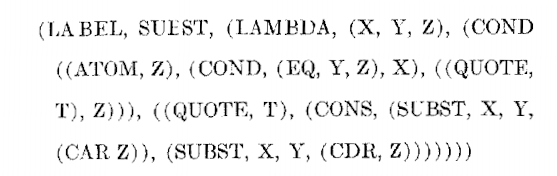
\includegraphics[scale=0.6]{images/readable1.png}\pause\n
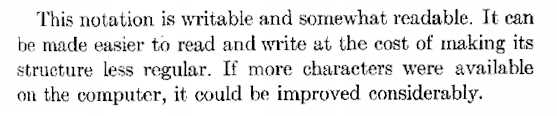
\includegraphics[scale=0.6]{images/readable2.png}
\end{figure}
\end{frame}


\begin{frame}
\frametitle{$apply$}

Funkcja $apply$ aplikuje S-wyrażenie $f$ reprezentujące S-funkcję $f'$ do listy argumentów $args$ postaci $(arg_1\,...\,arg_n)$.\pause

$$apply [f;args] = eval [cons [f; appq [args]]; NIL]$$ \n gdzie \n

\begin{equation*}
    \begin{gathered}    
    appq[m] = \\
    [null[m] \rightarrow NIL; \\
    T \rightarrow cons [list [QUOTE; car [m]]; appq [cdr [m]]]]
    \end{gathered}
\end{equation*}
\end{frame}


\begin{frame}
\frametitle{$eval$}

\begin{description}
    \item $eval[e;a] = [$ \pause
    \item \quad $atom[e] \rightarrow assoc[e; a]$ \pause
    \item \quad $atom[car[e]] \rightarrow [$ \pause
    \item \quad\quad $eq[car[e]; QUOTE] \rightarrow cadr[e];$ \pause
    \item \quad\quad $eq[car[e]; ATOM] \rightarrow atom[eval[cadr[e];a]];$\pause
    \item \quad\quad $eq[car[e]; EQ]
                      \rightarrow eval[cadr [e];a]=eval[caddr[e];a];$\pause
    \item \quad\quad $eq[car[e]; COND] \rightarrow evcon[cdr [e]; a];$\pause
    \item \quad\quad $eq[car [e]; CAR] \rightarrow car[eval[cadr[e];a]];$\pause
    \item \quad\quad $eq[car [e]; CDR] \rightarrow cdr[eval[cadr[e];a]];$\pause
    \item \quad\quad $eq[car[e];CONS] \rightarrow $ \n
          \quad\quad\quad$cons[eval[cadr[e];a];eval[caddr[e];a]];$\pause
    \item \quad\quad $T\rightarrow eval[cons [assoc[car [e];a]; evlis[cdr [e];a]
                    ];a]];$
\end{description}
\end{frame}


\begin{frame}
\frametitle{$eval$ cd.}
\begin{description}
    \item \quad $eq [caar [e]; LABEL] \rightarrow$ \n
          \quad\quad $[eval [cons[caddar [e]; cdr [e]];$ \n 
          \quad\quad $cons[list [cadar [e]; car[e]; a]];$\pause
    \item \quad $eq [caar [e]; LAMBDA] \rightarrow$ \n
          \quad\quad $eval[caddar [e]; append[pair[cadar[e]; evlis[cdr [e]; a]; a]]$ 
    \item $]$\pause
\end{description}

gdzie

$evcon[e;a] = [eval [caar [e];a] \rightarrow eval [cadar [e]; a];  T \rightarrow evcon[cdr[e];a]]$

\n

$evlis[m;a] = [null [m] \rightarrow NIL; T \rightarrow cons[eval[car[m];a];evlis[cdr[m];a]]]$
\end{frame}


\begin{frame}
\frametitle{Funkcje wyższego rzędu}
\pause

\begin{figure}
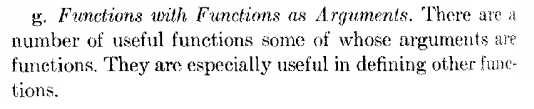
\includegraphics[scale=2.3]{images/higher-order-functions.png}
\end{figure}
\pause

\begin{description}
    \item $maplist[x;f] = [$
    \item \quad $null[x] \rightarrow NIL;$
    \item \quad $T \rightarrow cons[f[x]; maplist[cdr [x]; f]]]$
\end{description}
\pause\n
\begin{description}
    \item $search[x;p;f;u] = [$
    \item \quad $null [x] \rightarrow u;$
    \item \quad $p[x] \rightarrow f[x]$;
    \item \quad $T \rightarrow search [cdr [x]; p; f; u]]$
\end{description}
\end{frame}


\begin{frame}
\begin{figure}
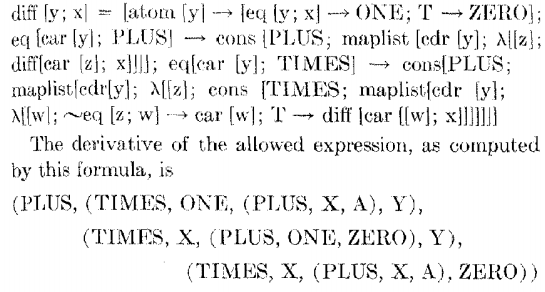
\includegraphics[scale=0.6]{images/diff.png}
\caption{Funkcja obliczająca pochodne funkcji zaaplikowana do wyrażenia $
         (TIMES, X, (PLUS, X, A), Y)$}
\end{figure}
\end{frame}


\begin{frame}
\frametitle{Reprezentacja S-wyrażeń w pamięci}
\pause
\begin{figure}
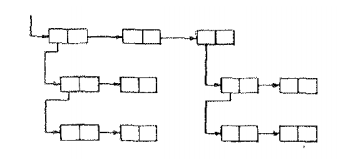
\includegraphics[scale=0.4]{images/list-layout-a.png}
\end{figure}
Lista jest zbiorem słów maszynowych zaaranżowanych w sposób podobny jak na powyższym rysunku. 
Każde słowo jest reprezentowane jako jeden z podzielonych na pół prostokątów.
\pause

\n
Każde słowo dzieli się na dwa pola: lewe $address$ oraz prawe $decrement$.
\pause
\end{frame}


\begin{frame}
\frametitle{Reprezentacja S-wyrażeń w pamięci}
\begin{columns}
\column{0.5\textwidth}
\begin{figure}
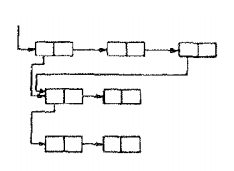
\includegraphics[scale=2.0]{images/list-layout-b.png}
\end{figure}
Jedna podstruktura może pojawiać się więcej niż w jednym miejscu w strukturze...
\pause
\column{0.5\textwidth}
\begin{figure}
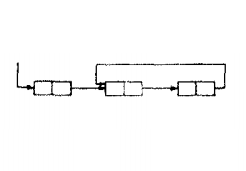
\includegraphics[scale=2.0]{images/list-layout-c.png}
\end{figure}
...ale struktury nie mogą zawierać cyklów.
\end{columns}
\end{frame}


\begin{frame}[label=current]
\frametitle{Reprezentacja S-wyrażeń cd.}




\end{frame}


%==============================================================================%

\section{Pierwsze implementacje}

\begin{frame}
\end{frame}

%==============================================================================%

\section{Być może coś więcej (Lisp-maszyny, Scheme)}
\begin{frame}
\end{frame}

\end{document}
